\documentclass[preprint,5p, 10pt, times]{elsarticle}

\usepackage{color, colortbl}

\usepackage{multirow}
\usepackage{array}
\usepackage{pifont}
\usepackage{ifsym}
\usepackage{tabu}
\newcommand\T{\rule{0pt}{2.6ex}}      
\newcommand\B{\rule[-1.2ex]{0pt}{0pt}}
\usepackage{upquote}
\usepackage{booktabs}
\usepackage{tabularx}
\usepackage{array}
\usepackage[table]{xcolor}
\usepackage{booktabs}
\usepackage{makecell}
\usepackage{array}

\definecolor{scoregreen}{RGB}{214,230,205}
\definecolor{scoreyellow}{RGB}{240,232,190}
\definecolor{scorered}{RGB}{236,213,205}

\newcommand{\good}[1]{\cellcolor{scoregreen}#1}
\newcommand{\medscore}[1]{\cellcolor{scoreyellow}#1}
\newcommand{\low}[1]{\cellcolor{scorered}#1}

\newcommand\DoTOC[1]{
    \section*{#1}
    \addcontentsline{dotoc}{section}{#1}
    \markboth{#1}{#1}}

\usepackage{mdframed}
\usepackage[dvipsnames, table]{xcolor}
\usepackage{amssymb}
\usepackage{color}
\usepackage{subcaption}
\definecolor{Green}{RGB}{0,102,102}
\usepackage{tikz}

\journal{npj Digital Medicine}
\usepackage{titlesec}

\titleformat{\section}
{\color{black}\normalfont\large\bf\sffamily}
{\color{black}\thesection}{1em}{}
\usepackage[colorlinks,citecolor=blue,urlcolor=blue,bookmarks=false,hypertexnames=true]{hyperref} 
%--------------------

\titleformat{\subsection}
{\color{black}\normalfont\normalsize\bf\sffamily}
{\color{black}\thesubsection}{1em}{}{}

\usepackage[superscript,biblabel, compress]{cite}
\usepackage{titletoc}

\newcommand\DoToC{%
  \startcontents
  \printcontents{}{1}{\textbf{Contents}\vskip3pt\hrule\vskip5pt}
  \vskip3pt\hrule\vskip5pt
}
%To have multiple reference sets
\usepackage[labeled,resetlabels]{multibib}
\newcites{a}{ }

\usepackage{tabu}

\begin{document}
\sloppy

\begin{frontmatter}

\title{\Large \bf Fedlify: An Agentic Federated Learning Platform for Health AI}

\author{
    \textbf{\fontsize{11pt}{13.3pt}\selectfont{
    Omid Jafarinezhad\textsuperscript{1}, 
    Mohammad Noaeen\textsuperscript{1},\\  
    Aviv Shachak\textsuperscript{1,3}, 
    Behrouz Far\textsuperscript{4}, and Zahra Shakeri\textsuperscript{1,3,5,*}}} 
    \\
    \small\normalfont
    \textsuperscript{1}{Institute of Health Policy, Management and Evaluation, Dalla Lana School of Public Health, University of Toronto, Toronto, Canada} \\
    \textsuperscript{3}{Faculty of Information, University of Toronto, Toronto, Canada} \\
\textsuperscript{4}{Department of Electrical and Software Engineering, University of Calgary, Calgary, Canada} \\
\textsuperscript{5}{Schwartz Reisman Institute, University of Toronto, Toronto, Canada} \\
    \textsuperscript{*}{Corresponding author, zahra.shakeri@utoronto.ca}
}


\begin{abstract}
\centering\begin{minipage}{\dimexpr\paperwidth-3cm}


\textcolor{red}{context, gap, Fedlify, approach, key results, and impact.}

\end{minipage}

\end{abstract}


\end{frontmatter}

\section*{Introduction}
\label{S:Intro}

\textcolor{blue}{\textbf{[Health AI and the data challenge.]}}
Health artificial intelligence (AI) increasingly depends on patient-level data such as electronic health records, medical imaging, genomics, and biosignals to detect complex clinical patterns and support precision medicine \cite{moor2023foundation, acosta2022multimodal,tu2024towards}. 
However, the development of reliable and generalizable health AI models often requires collaboration across multiple institutions \cite{tayebi2023enhancing,rockenschaub2024impact,li2023model}. 
In practice, such collaboration remains difficult due to privacy regulations, governance requirements, and institutional barriers surrounding the sharing of sensitive health data. 
These challenges are further amplified in countries with decentralized healthcare governance, such as Canada, Germany, and Australia, where jurisdiction-specific regulatory frameworks and fragmented data infrastructures add layers of complexity.
\cite{alami2024understanding,hassan2024barriers}.
As a result, many health AI models are trained on single-institution datasets, which constrains their generalizability and clinical reliability across diverse patient populations\cite{suleman2025assessing, arun2025systematic,pandian2025generalizing,naderian2025systematic}.

\textcolor{blue}{\textbf{[Federated learning and its adoption gap.]}}
Federated learning (FL) is a novel paradigm for privacy-preserving machine learning that addresses part of this problem by allowing institutions to collaboratively train models without transferring raw data.
Rather than moving sensitive data to a central location, FL enables institutions to collaboratively train AI models while data remain securely under local control\cite{mcmahan2017communication,ur2021federated}. 
This approach is especially relevant in health research, where privacy, trust, and institutional accountability are essential\cite{teo2024federated,guan2024federated}. 
In principle, FL enables inter-institutional collaboration in contexts where sharing raw health data is constrained by privacy regulations.
In practice, however, its adoption in health research remains limited.
\textcolor{blue}{Jafarinezhad et al.} reviewed 3,100 patient-level AI studies published between 2018 and 2025 and found that only 5\% of multicenter studies employed FL. Similarly, Teo et al. reviewed 612 healthcare FL studies and reported that most remained proof-of-concept, with only 5.2\% describing real-world applications \cite{teo2024federated}.
Most health AI collaboration still depends on centralized data aggregation, even when this creates governance difficulties or excludes institutions that cannot transfer patient data. This suggests that the key challenge is no longer whether FL works technically, but how it can be implemented in ways that align with the operational and governance realities of health AI research.

\textcolor{red}{\textbf{The core limitation is operational, not algorithmic.}} Existing federated learning research focuses on algorithms and frameworks, while key system-level challenges such as workflow orchestration, governance integration, and reproducibility remain unaddressed.

\textcolor{red}{\textbf{Increasing workflow complexity requires structured coordination.}} As federated studies grow in scale, coordinating multi-step processes across sites becomes increasingly difficult without dedicated system support.

\textcolor{red}{\textbf{Fedlify: an agentic federated learning platform.}} We present Fedlify, a platform designed to support the full lifecycle of federated health AI studies through structured workflows, embedded governance, and reproducible execution.

\textcolor{red}{\textbf{Contributions.}} This work introduces a system architecture for federated learning in health AI, a governance-aware workflow model, a deployable platform for heterogeneous environments, and a system-level evaluation using simulated multi-site studies.

% Over the past few years, AI agents powered by large language models have begun to emerge \textbf{REF}. These agents are software systems that perceive their environment, reason about it, and take actions on their own to achieve user-defined goals. With added perception and execution components, large language models no longer only respond to prompts. They act through agents that plan, store information, and interact across digital systems \textbf{REF}. These agents can also work together to achieve complex objectives \textbf{REF}.

% Two main forces drive the shift toward agent-based systems. First, AI assistants now handle complex, multi-step tasks in areas such as research \textbf{REF}, software development \textbf{REF}, \textbf{OTHER}. These agents no longer act as reactive tools that answer isolated prompts. They operate as proactive collaborators that plan, reason, and carry out actions over time. Second, users now trust these systems more and often delegate full workflows to them. These workflows can last minutes, hours, or even days \textbf{REF}. This increased trust in agent autonomy creates new expectations and calls for new interfaces. As a result, it changes how people use and experience ....

% background and review of existing frameworks with comparison in a table


% -----------------------------------------------------
% -----------------------------------------------------


%-----------------------------------------------------
%-----------------------------------------------------
\section*{Results}

\textcolor{blue}{\textbf{[Comparison of existing FL frameworks.]}}
To examine how well current FL frameworks align with the requirements of real-world multi-site health AI studies, we compared the selected FL frameworks against the criteria defined in Table \ref{tab:comparison_criteria}. The results, summarized in Table \ref{tab:fl_framework_comparison}, showed that the clearest differences did not arise from the federated training loop itself, but from deployment readiness, workflow orchestration, traceability, and governance.
This pattern suggests that the main gaps in the field are not primarily algorithmic, but relate more to the operational, infrastructural, and organizational conditions required for real-world multi-site use.

FL Frameworks positioned for production or institutional collaboration provided the most complete documented support across the comparison dimensions. 
FATE is presented as an industrial-grade platform for privacy-preserving collaborative learning, with an emphasis on large-scale distributed collaboration, secure computation protocols, end-to-end modules, and usability\cite{liu2021fate}. 
NVFlare is framed as a simulation-to-real-world federated learning SDK that supports privacy-preserving workflows across enterprises and highlights deployment, failover, multitasking, and extensibility\cite{roth2022nvidia}. 
Substra is described as a privacy-preserving, traceable, and collaborative framework with advanced permission controls and explicit traceability of distributed computation\cite{galtier2019substra}. 
OpenFL likewise extends beyond research simulation by emphasizing production migration, real-world scalability, trusted execution, and healthcare federations\cite{reina2021openfl}. 
Despite these strengths, their support remains concentrated at the level of federated execution and deployment. They move beyond training abstractions, but they do not fully resolve the higher-level requirements of reusable study coordination, governance-aware administration, and traceable multi-site workflow management that become central in real-world health AI collaboration.


Another group of frameworks offered broad technical breadth, but provided less support for governance-aware deployment across multiple sites and for system-level reuse of the collaboration process across different networks of participating institutions.
Flower supported large-scale experimentation, heterogeneity handling, and migration from simulation to real devices, which places it beyond a purely experimental environment \cite{beutel2020flower}. 
Its contribution lies primarily in scalable experimentation and execution, while the governance structures needed for institutional collaboration remain limited.
TensorFlow Federated (TFF) \cite{bonawitz2019towards} and FLGo \cite{wang2023flgo} show a similar limitation through different design priorities. TFF presents a high-scale production system for synchronized cross-device learning in a TensorFlow-based mobile environment, whereas FLGo is designed around customizability, benchmarking, reproducibility, and experimental shareability.
EasyFL makes a different contribution by lowering the entry barrier to experimentation through low-code abstractions, tracking, and deployment convenience\cite{zhuang2022easyfl}. 
These frameworks make important technical contributions, but their focus remains on experimentation and developer usability rather than on the system-level support needed to organize, govern, and sustain multi-site health AI collaboration.

FedOps\cite{moon2024fedops,yang2023flscalize}, FLScalize\cite{beltran2024fedstellar}, and Fedstellar\cite{beltran2024fedstellar} shift attention to a different layer of the problem. They show that FL becomes difficult to sustain when deployment, lifecycle management, heterogeneity, and monitoring must be managed across real environments. FLScalize focuses on lifecycle management for moving models and data into federated settings, FedOps adds operational and heterogeneity-management support, and Fedstellar broadens the design space through support for centralized and decentralized topologies within one platform. Even with these advances, broader requirements for governance-aware collaboration, cross-site coordination, traceability, and reusable study-level management remain only partly integrated, particularly in institutional and healthcare settings. 

Using GitHub commit recency as a practical maintenance indicator, the selected frameworks could be grouped into those with recent active development, with a last commit within the past year, and those with a less recent maintenance profile, with the last visible commit more than one year old. Although commit recency does not by itself determine software quality or readiness, it provides a useful signal of ongoing project activity and support.
TFF, Flower, NVFlare, OpenFL, IBM Federated Learning, FLGo, and FedOps showed recent development within the past year. FATE, FedML, PaddleFL, SubstraFL, EasyFL, and Fedstellar did not show publicly visible commit activity within the past year.


The evaluation revealed a consistent distinction between frameworks that can execute a federated learning study and frameworks that can support repeated multi-institutional studies as an operational platform. For a single study, several production-oriented FL frameworks provided documented support for installation, configuration, execution control, site connectivity, and project-level coordination. In other words, they could help a team set up and run one federated study across participating sites. Their support was more limited, however, when the comparison shifted to tasks that recur across studies, such as reusing the same collaboration structure in a new institutional network, managing users and roles, preserving workflow records across the study lifecycle, and re-establishing governance and administrative controls in heterogeneous health data environments. At this broader level, fewer frameworks provided clear support for reusable study coordination, governance-aware administration, and workflow traceability beyond the boundaries of a single project.
Capability coverage and communication support were also documented in many frameworks, although the breadth of support varied. 
Governance remained the weakest and least standardized dimension.

These findings have direct design implications for Fedlify. The comparison does not suggest that current FL frameworks are technically weak. 
Several provide mature support for federated training, security mechanisms, and operational deployment. 
What remains less developed is the layer required to make these capabilities usable in governed, multi-site health AI studies. 
The main gap is therefore not the absence of FL runtimes. It is the absence of a platform layer that can structure workflows, preserve traceability, and align collaboration with institutional governance requirements. 
These observations motivate Fedlify’s emphasis on governance-aware coordination, reusable study management, and system-level support beyond federated execution alone.

\textcolor{blue}{\textbf{[Agreement and adjudication analysis.]}}
To strengthen the transparency of the framework comparison, the evaluation workflow was extended to support independent evidence-locked review by two large language model (LLM) assistive coders, GPT-5.5 and Claude Sonnet, alongside the human-coded baseline. 
The workflow records the exact evidence packets, prompts, model identifiers, raw responses, normalized scores, and adjudication flags in a derived audit workbook. 
Agreement is summarized using criterion-level mean absolute score differences and band disagreements across the human--GPT, human--Claude, and GPT--Claude comparisons. 
Any model--human score difference of three or more points, or any disagreement between limited, partial, and full support bands, is flagged for human adjudication before final scores are used in Table~\ref{tab:fl_framework_comparison}.
Because the LLM outputs are used as assistive evidence rather than as ground truth, unresolved disagreement is resolved conservatively against the underlying source evidence.

% \begin{figure*}
%     \centering
%     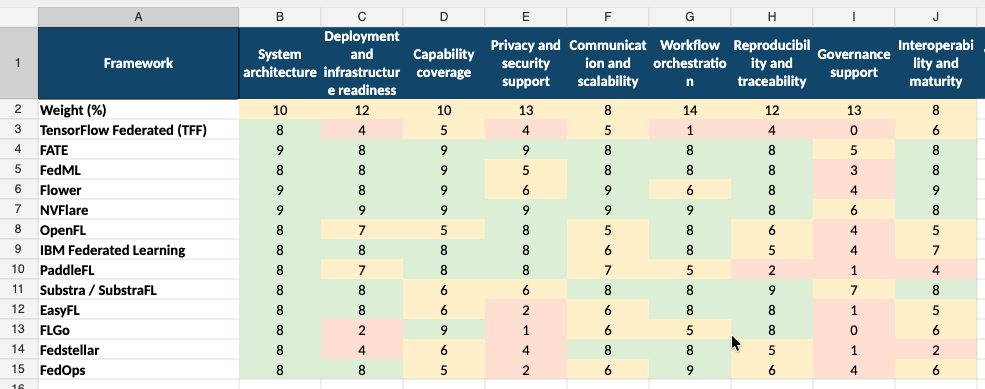
\includegraphics[width=1\linewidth]{FL_table.png}
%     \caption{Enter Caption}
%     \label{fig:placeholder}
% \end{figure*}

\begin{table*}[t]
\centering
\renewcommand{\arraystretch}{1.15}
\setlength{\tabcolsep}{4pt}
\caption{\textbf{Comparison of federated learning frameworks across evaluation dimensions.} Selected frameworks were compared across technical, operational, and governance-related criteria relevant to multi-site health AI studies. Green denotes full support, yellow denotes partial support, and red denotes limited support.}
\label{tab:fl_framework_comparison}
\resizebox{\textwidth}{!}{%
\begin{tabular}{lccccccccc}
\toprule
\textbf{Framework} &
\makecell{\textbf{System}\\\textbf{architecture}} &
\makecell{\textbf{Deployment and}\\\textbf{infrastructure}\\\textbf{readiness}} &
\makecell{\textbf{Capability}\\\textbf{coverage}} &
\makecell{\textbf{Privacy and}\\\textbf{security}\\\textbf{support}} &
\makecell{\textbf{Communication}\\\textbf{and}\\\textbf{scalability}} &
\makecell{\textbf{Workflow}\\\textbf{orchestration}} &
\makecell{\textbf{Reproducibility}\\\textbf{and}\\\textbf{traceability}} &
\makecell{\textbf{Governance}\\\textbf{support}} &
\makecell{\textbf{Interoperability}\\\textbf{and}\\\textbf{maturity}} \\
\midrule

TensorFlow Federated (TFF)\cite{bonawitz2019towards}
& \good{} & \low{} & \medscore{} & \low{} & \medscore{} & \low{} & \low{} & \low{} & \medscore{} \\

FATE\cite{liu2021fate}
& \good{} & \good{} & \good{} & \good{} & \good{} & \good{} & \good{} & \medscore{} & \good{} \\

FedML\cite{he2020fedml}
& \good{} & \good{} & \good{} & \medscore{} & \good{} & \good{} & \good{} & \low{} & \good{} \\

Flower \cite{beutel2020flower}
& \good{} & \good{} & \good{} & \medscore{} & \good{} & \medscore{} & \good{} & \low{} & \good{} \\

NVFlare\cite{roth2022nvidia}
& \good{} & \good{} & \good{} & \good{} & \good{} & \good{} & \good{} & \medscore{} & \good{} \\

OpenFL\cite{reina2021openfl}
& \good{} & \medscore{} & \medscore{} & \good{} & \medscore{} & \good{} & \medscore{} & \low{} & \medscore{} \\

IBM Federated Learning\cite{ludwig2020ibm}
& \good{} & \good{} & \good{} & \good{} & \medscore{} & \good{} & \medscore{} & \low{} & \medscore{} \\

PaddleFL\cite{paddlefl}
& \good{} & \medscore{} & \good{} & \good{} & \medscore{} & \medscore{} & \low{} & \low{} & \low{} \\

Substra / SubstraFL\cite{galtier2019substra}
& \good{} & \good{} & \medscore{} & \medscore{} & \good{} & \good{} & \good{} & \medscore{} & \good{} \\

EasyFL\cite{zhuang2022easyfl}
& \good{} & \good{} & \medscore{} & \low{} & \medscore{} & \good{} & \good{} & \low{} & \medscore{} \\

FLGo\cite{wang2023flgo}
& \good{} & \low{} & \good{} & \low{} & \medscore{} & \medscore{} & \good{} & \low{} & \medscore{} \\

Fedstellar\cite{beltran2024fedstellar}
& \good{} & \low{} & \medscore{} & \low{} & \good{} & \good{} & \medscore{} & \low{} & \low{} \\

FedOps\cite{moon2024fedops,yang2023flscalize}
& \good{} & \good{} & \medscore{} & \low{} & \medscore{} & \good{} & \medscore{} & \low{} & \medscore{} \\

\bottomrule
\end{tabular}%
}
\end{table*}


\textcolor{blue}{\textbf{[Proposed agentic framework for federated health AI.]}}
Based on the gaps identified in the framework comparison, we propose an agentic framework for Fedlify that treats federated learning as a governed workflow rather than only as a training procedure. 
The framework follows the modular structure used in contemporary LLM-agent systems: a bounded workspace, task-specific instructions, memory over approved project context, tool-mediated action, validation, and human feedback \cite{wang2024surveyagents,yao2023react,schick2023toolformer}. 
This design is also aligned with health AI governance guidance that emphasizes human oversight, transparency, accountability, data protection, and risk management \cite{who2021ethicsaihealth,nist2023airmf}. 
In Fedlify, the chatbot is therefore not only a help interface. It is the structured intake and coordination interface through which a researcher describes a study, the system identifies missing operational requirements, and specialized skills produce draft artifacts for review. 
The agent may gather metadata, generate plans, generate configuration, and prepare code from approved templates, but it cannot approve a collaboration, access patient-level data, execute a study, release site kits, or override institutional governance.

\begin{table*}[t]
\centering
\caption{\textbf{Minimum evidence-backed taxonomy used by the Fedlify agent.} The chatbot records these fields before workflow planning and code generation so that outputs are grounded in the clinical FL setting rather than in generic pipeline defaults.}
\label{tab:fedlify_agent_taxonomy}
\tiny
\setlength{\tabcolsep}{3pt}
\renewcommand{\arraystretch}{1.16}
\begin{tabularx}{\textwidth}{
>{\raggedright\arraybackslash}p{2.6cm}
>{\raggedright\arraybackslash}X
>{\raggedright\arraybackslash}X
>{\raggedright\arraybackslash}X}
\toprule
\textbf{Aspect} & \textbf{Agent instruction} & \textbf{Example structured answer} & \textbf{Evidence basis} \\
\midrule
\textbf{Collaboration setting}
& Classify whether participants are stable institutions, dynamic devices/wearables, or a hybrid collaboration; record coordinator and participant roles.
& Cross-silo hospitals: two hospitals train locally and one academic center coordinates.
& Cross-silo/cross-device distinctions and health deployment coordination are emphasized in FL surveys and digital-health FL analyses \cite{kairouz2021advances,rieke2020future,eden2025scoping}. \\

\textbf{Data distribution}
& Determine whether data are horizontal, vertical, or partially overlapping; flag private linkage or transfer-learning needs before using standard FedAvg.
& Horizontal FL: different patients at each site with a shared feature dictionary and common label.
& Horizontal, vertical, and federated transfer learning are standard FL categories; medical surveys show data partition and heterogeneity affect feasibility \cite{yang2019federated,teo2024federated,choi2024survey}. \\

\textbf{Data modality}
& Map EHR/tabular, imaging, waveform, genomics, text, and wearable modalities to local data contracts, dependencies, synthetic fixtures, and validation checks.
& Medical imaging with local DICOM-to-tensor preprocessing; no images leave sites.
& Medical FL applications are commonly stratified by data type, with imaging, structured medical data, and multimodal settings requiring different controls \cite{choi2024survey,guan2024federated,kaissis2020secure}. \\

\textbf{System topology}
& Select centralized, decentralized/peer-to-peer, or hierarchical topology from the trust model, networking constraints, and governance responsibilities.
& Hierarchical aggregation: sites aggregate within a health network before global aggregation.
& FL system design and health FL deployment papers show topology affects trust, communication, failure handling, and orchestration \cite{kairouz2021advances,bonawitz2019towards,rieke2020future}. \\

\textbf{Privacy and security}
& Convert required controls such as secure aggregation, differential privacy, homomorphic encryption, hardware trust, and attack defenses into validation checks and stop conditions.
& Secure aggregation where supported, signed startup kits, threat review, no raw-data paths, and human release review.
& FL does not eliminate privacy risk; medical imaging and healthcare privacy reviews emphasize gradient leakage, inference, poisoning, cryptographic protection, and governance controls \cite{kaissis2020secure,who2021ethicsaihealth,nist2023airmf}. \\

\textbf{Training strategy}
& Choose synchronous, asynchronous, semi-asynchronous, or personalized FL based on site availability, compute heterogeneity, non-IID risk, and whether site-adapted models are needed.
& Personalized FL because sites have different patient populations and local calibration matters.
& Heterogeneous clients create stragglers and stale updates; personalized and asynchronous FL address irregular clients and non-IID data \cite{li2024fedcompass,ma2023asynchronous,kairouz2021advances}. \\

\textbf{Clinical application and disease area}
& Record diagnosis, prognosis, treatment support, clinical research, or operations; record disease category; require explicit endpoint definitions instead of inferring labels.
& Prognosis in critical care: ICU mortality prediction using structured EHR data.
& Digital-health FL and medical application surveys categorize studies by clinical purpose, disease target, and data type \cite{rieke2020future,choi2024survey,teo2024federated}. \\

\textbf{Challenge profile}
& Convert non-IID data, small or imbalanced cohorts, compute/network limits, deployment complexity, privacy-utility trade-offs, reproducibility, benchmarking, fairness, incentives, and governance into warnings, validation tasks, or approval gates.
& Non-IID data, small site cohorts, limited compute, fairness risk, and benchmark reporting required.
& Public-health FL, benchmarking, governance, and bias surveys document deployment barriers, reproducibility needs, and fairness risks \cite{shah2025publichealthfl,karargyris2023medperf,eden2025scoping,benarba2025bias}. \\
\bottomrule
\end{tabularx}
\end{table*}

\begin{table*}[t]
\centering
\caption{\textbf{Concrete agentic skills proposed for Fedlify.} Each skill is defined as a bounded implementation unit with explicit triggers, inputs, instructions, output artifacts, validation checks, guardrails, and literature basis.}
\label{tab:fedlify_agentic_framework}
\tiny
\setlength{\tabcolsep}{2.5pt}
\renewcommand{\arraystretch}{1.18}
\begin{tabularx}{\textwidth}{
>{\raggedright\arraybackslash}p{2.4cm}
>{\raggedright\arraybackslash}p{2.7cm}
>{\raggedright\arraybackslash}X
>{\raggedright\arraybackslash}X
>{\raggedright\arraybackslash}X}
\toprule
\textbf{Skill} & \textbf{Trigger and required inputs} & \textbf{Skill instruction} & \textbf{Output and validation} & \textbf{Guardrails and evidence basis} \\
\midrule

\textbf{Study intake and eligibility triage}
& Triggered when a user starts a study from the chatbot. Required inputs are a research goal, clinical/biomedical task, data modality, intended participating sites, outcome/label definition, and known governance constraints.
& Ask only for the minimum information needed to create a structured study record. Extract the task, cohort, modality, label, FL motivation, participating institutions, expected outputs, and missing requirements. Classify the study as ready, incomplete, or not yet suitable for FL.
& Produces a study-intake record, missing-information list, and readiness status. Validation checks require non-empty task, modality, site list, outcome definition, and governance contact before workflow planning can start.
& The agent must not request or store raw patient records, identifiers, credentials, or secrets. Intake is metadata-only and must be confirmed by the user. This responds to evidence that healthcare FL failures often arise from organizational, regulatory, and socio-technical readiness gaps rather than training code alone \cite{schoenpflug2025navigating,peltonen2026federated,eden2025scoping}. \\
\addlinespace[3pt]

\textbf{Data-readiness and federation design}
& Triggered after intake when sites describe local data availability. Required inputs are aggregate counts, modality, feature/schema description, label availability, missingness summary, data partition assumptions, and site constraints.
& Convert site descriptions into a data-readiness matrix. Identify whether the study is horizontal FL, vertical FL, federated transfer learning, or not yet alignable. Flag non-IID risk, incompatible labels, missing feature definitions, small site sample sizes, and modality-specific constraints.
& Produces a site-by-site readiness matrix, federation-design recommendation, and data-gap report. Validation checks confirm that label definitions, feature/schema descriptions, and split assumptions are consistent across sites before code generation.
& Only metadata, aggregate counts, and data dictionaries are accepted. The agent cannot infer clinical labels or harmonize variables without user approval. This skill is grounded in healthcare FL reviews showing that architecture, partition setting, modality, privacy reporting, and heterogeneity shape feasibility \cite{teo2024federated,guan2024federated,chai2024survey}. \\
\addlinespace[3pt]

\textbf{Governance, privacy, and safety review}
& Triggered before workflow freeze or when a site, data source, or execution mode changes. Required inputs are institutional roles, data-use constraints, privacy controls, security requirements, and approval status.
& Map the study to governance requirements: procedural controls, stakeholder responsibilities, access roles, privacy-preserving mechanisms, audit expectations, and unresolved ethics or data-sharing issues.
& Produces a governance checklist, privacy/security checklist, role matrix, and blocker log. Validation checks require named responsible users, approved site roles, and a documented decision for privacy/security mechanisms before kit release.
& The agent cannot waive policy, ethics, privacy, or security requirements. Any unresolved governance blocker stops progression. This follows healthcare FL governance evidence and general AI risk-management guidance emphasizing accountability, transparency, privacy, human oversight, and lifecycle risk management \cite{eden2025scoping,who2021ethicsaihealth,nist2023airmf,jimenez2026security,zhao2025federation}. \\
\addlinespace[3pt]

\textbf{Workflow planning and orchestration}
& Triggered when intake, data readiness, and governance checks are complete. Required inputs are approved study metadata, site readiness, selected FL framework/template, resource constraints, and governance checkpoints.
& Produce a workflow state machine for collaboration creation, site onboarding, configuration, approval, workflow freeze, kit generation, local execution, aggregation, monitoring, completion, and reporting. Represent dependencies explicitly.
& Produces a workflow plan, state transition list, approval checklist, and runbook. Validation checks ensure every execution step has an owner, precondition, expected artifact, and rollback/escalation path.
& The agent can draft a workflow but cannot mark approvals complete or execute steps. Human approval gates remain mandatory before workflow freeze and execution. This is motivated by real-world FL deployment reports emphasizing provisioning, networking, coordination, monitoring, partner management, and provenance \cite{schoenpflug2025navigating,schlegel2026lowering,peltonen2026federated}. \\
\addlinespace[3pt]

\textbf{Template-bound code and configuration generation}
& Triggered only after workflow freeze. Required inputs are approved workflow plan, framework choice, site manifests, resource settings, data schema metadata, and selected model/pipeline template.
& Generate only bounded artifacts: framework configuration, site manifests, container instructions, data-loader skeletons, validation scripts, and execution-kit contents. Use approved templates and explicit user choices rather than open-ended code synthesis.
& Produces a code/configuration bundle, manifest, and diff-style summary. Validation checks include schema validation, no embedded secrets, no patient-level data paths in prompts, template provenance, deterministic artifact names, and dry-run validation where possible.
& The agent cannot invent new FL algorithms, add unapproved dependencies, include credentials, or release kits without approval. Tool-mediated generation follows agent research showing that LLMs are more useful when reasoning is connected to external tools and APIs, but bounded by validation \cite{yao2023react,schick2023toolformer,nist2023airmf}. \\
\addlinespace[3pt]

\textbf{Monitoring, failure triage, and remediation planning}
& Triggered during site setup, local execution, or aggregation. Required inputs are logs, site heartbeat/status, validation output, execution stage, and previous approved plan.
& Summarize what happened, classify the failure, identify the affected site/stage/artifact, and propose bounded remediation steps. Distinguish infrastructure, configuration, data-readiness, governance, and framework-runtime failures.
& Produces a monitoring summary, failure classification, and remediation proposal. Validation checks compare observed state with the approved workflow state machine and require human confirmation for high-impact remediation.
& The agent cannot silently retry steps that affect privacy, permissions, data movement, or released artifacts. It can recommend but not override site controls. This responds to deployment evidence that coordination, monitoring, networking, and failure handling remain major barriers in real FL settings \cite{schoenpflug2025navigating,moon2024fedops}. \\
\addlinespace[3pt]

\textbf{Reproducibility, audit, and report drafting}
& Triggered after workflow freeze, after kit generation, during execution, and at study completion. Required inputs are approved intake, workflow version, artifact hashes, validation output, execution events, and final run metadata.
& Build the reproducibility package: record who approved what, which configuration was used, which artifacts were generated, which sites participated, what validation passed, and what outputs were produced. Draft methods/report text from observed evidence only.
& Produces audit trail, reproducibility package, artifact index, and methods/report draft. Validation checks require artifact hashes, timestamps, role attribution, and distinction between observed facts and generated narrative.
& Audit logs exclude raw patient data. The agent cannot fabricate missing provenance or convert unverified summaries into results. This skill addresses literature emphasizing traceability, provenance, interoperability, and repeatable workflow records for biomedical FL \cite{schlegel2026lowering,chavero2026federated,chai2024survey,nist2023airmf}. \\
\bottomrule
\end{tabularx}
\end{table*}

This proposed framework defines the implementation target for the next Fedlify chatbot workflow. 
Each skill is implemented as a versioned skill card rather than as an unrestricted chat prompt. 
The runtime contract for each card records the trigger, required inputs, agent instruction, allowed tools, output schema, validation tests, stop conditions, human approval gate, and evidence basis. 
The agent-instruction field defines the concrete action the model is allowed to perform, while the guardrail fields define what must be refused, escalated, or blocked before the workflow can advance. 
The chatbot first gathers enough metadata to decide whether a study is ready for FL. 
The skill router then selects the next skill based on missing information and workflow state. 
Only after intake, data readiness, and governance checks are complete can the workflow planner prepare an executable study plan. 
Only after workflow freeze can the code-generation skill produce site-specific artifacts. 
The key design principle is controlled agency: the agent accelerates data gathering, planning, code generation, validation, and reporting, while human approval, institutional governance, local data control, and reproducibility records constrain every execution-relevant action.



\textcolor{red}{\textbf{Overview of system capabilities.}} Fedlify enables end-to-end coordination of federated studies, including study configuration, site onboarding, execution, and result aggregation.

\textcolor{red}{\textbf{End-to-end workflow execution.}} The system supports the full lifecycle of federated learning workflows, from study setup to multi-site training and aggregation, without requiring manual coordination between participating sites.

\textcolor{red}{\textbf{Application/Case study: multi-site federated study.}} We conducted a simulated multi-site study reflecting real-world health AI constraints, where Fedlify managed study configuration, site participation, orchestration, and execution. The workflow was completed successfully across all sites, demonstrating reduced coordination overhead and consistent execution.

\textcolor{red}{\textbf{Reproducibility and system stability.}} Repeated executions of the same workflow produced consistent results, supported by structured logging, configuration versioning, and traceable execution steps.


% -----------------------------------------------------
% -----------------------------------------------------
\section*{Discussion}

\textcolor{red}{\textbf{[Barriers to federated learning adoption.]}}
The pattern observed in our comparison is consistent with recent literature on real-world FL implementation. Recent work in healthcare FL has emphasized that practical limitations often arise not from the federated training loop itself, but from the surrounding conditions required to organize, govern, deploy, and sustain collaboration across institutions. 
Peltonen and Chomutare argue, on the basis of a 3-year Nordic–Baltic health data network spanning 5 countries and 9 institutions, that the main barriers to healthcare FL are often organizational, regulatory, and socio-technical rather than purely technical\cite{peltonen2026federated}. 
Eden et al. likewise show that governance in healthcare FL extends beyond computation to procedural, relational, and structural mechanisms, which suggests that successful deployment depends on how collaboration is organized and governed across sites\cite{eden2025scoping}. 
In a real-world computational pathology case study, Schoenpflug et al.  report that site provisioning, networking, coordination, and monitoring remain major practical challenges during deployment\cite{schoenpflug2025navigating}. 
Schlegel et al. similarly identify collaboration management, partner matching, and provenance tracking as persistent barriers that limit usable FL in practice\cite{schlegel2026lowering}.
These findings support our interpretation that meaningful differences across current FL frameworks come more from operational and governance requirements than from training functionality alone.


....

\textbf{How Fedlify addresses these challenges.} Fedlify is designed around two complementary directions intended to better align federated learning with real-world multi-site study requirements. One is a governance-oriented application layer, planned to support functions such as user management, role management, access control, and related forms of administrative oversight typical of data-intensive applications. The other is an agentic coordination approach, intended to help manage the technical complexity of federated workflows through support for configuration, coordination, monitoring, and execution across sites. Together, these design choices position Fedlify as more than a training runtime alone, and instead as a platform for organizing both the operational and governance-related dimensions of federated health AI studies..

\textcolor{red}{\textbf{Implications for health AI research.}} The platform enables more practical and scalable multi-institutional studies, supports reproducibility and governance-aware collaboration in real-world settings.

\textcolor{red}{\textbf{Limitations.}} This study was conducted in a simulated multi-site environment without live clinical deployment, and evaluation was limited to system-level validation.

\textcolor{red}{\textbf{Future work.}} Future efforts will focus on deployment in real healthcare environments, integration with clinical systems, and ....

% \textquotesingle\␣


% -----------------------------------------------------
% -----------------------------------------------------
\section*{Methods}
\textcolor{blue}{\textbf{Evaluation criteria.}}
We derived the evaluation criteria from prior literature on FL evaluation, healthcare implementation, governance, and biomedical software assessment to align the comparison with the requirements of real-world multi-institution health AI research. 
Chai et al. frame FL evaluation around utility, efficiency, and security and indicate that framework assessment cannot rely on predictive performance alone \cite{chai2024survey}.
Teo et al. characterize healthcare FL as technically uneven and translationally limited, with studies concentrated in a narrow set of architectures, partition settings, and application types, and with privacy safeguards reported inconsistently \cite{teo2024federated}.
Schoenpflug et al. identify real deployments face limits in site provisioning, networking, coordination, and monitoring \cite{schoenpflug2025navigating}. 
Eden et al. characterize governance in healthcare FL in terms of procedural, relational, and structural mechanisms. \cite{eden2025scoping}.
At the software level, Chavero-Díez et al. report limited interoperability across current FL frameworks despite acceptable findability and reusability \cite{chavero2026federated}. 
Mehdi et al. identify architecture, deployment ease, scalability, and community support as recurring dimensions in framework comparison \cite{mehdi2025comprehensive}.
On this basis, we assessed the FL frameworks across the criteria shown in Table \ref{tab:comparison_criteria}, which cover system architecture, deployment readiness, capability coverage, privacy and security support, communication and scalability, workflow orchestration, reproducibility and traceability, governance support, and interoperability and maturity. This allowed the comparison to capture both core engineering properties and practical suitability for multi-site health AI studies.

\begin{table*}[t]
\centering
\caption{Comparison criteria used to evaluate federated learning frameworks for multi-site health AI studies
}
\label{tab:comparison_criteria}
\scriptsize
\setlength{\tabcolsep}{3pt}

\begin{tabularx}{\textwidth}{
>{\raggedright\arraybackslash}p{2.2cm}
>{\raggedright\arraybackslash}X
>{\raggedright\arraybackslash}X
>{\centering\arraybackslash}p{1.1cm}}
\toprule
\textbf{Criterion} & \textbf{Operational definition} & \textbf{Rationale} & \textbf{Key references} \\
\midrule

\textbf{System architecture}
& Overall coordination model, topology, modular structure, and degree of coupling to specific machine learning stacks.
& Architecture determines extensibility, heterogeneity support, trust assumptions, and the boundary between orchestration, execution, and site control. It also shapes deployment, security, and workflow integration across the framework.
& \cite{chai2024survey,mehdi2025comprehensive, antunes2022federated, mahmud2026survey, wang2022efficient} \\
\addlinespace[4pt]

\textbf{Deployment and infrastructure readiness}
& Ease of installation, packaging, configuration, and support for on-premise, cloud, edge, or hybrid environments.
& Multi-site federated learning studies depend on whether the system can be provisioned and operated across heterogeneous institutional infrastructures.
& \cite{zhang2022shifting,teo2024federated,schoenpflug2025navigating,mehdi2025comprehensive} \\
\addlinespace[4pt]

\textbf{Capability coverage}
& Supported training modes (e.g., synchronous and asynchronous), data partition settings (e.g., horizontal and vertical FL), FL settings and learning paradigms (e.g., federated transfer learning and personalized FL), aggregation strategies (e.g., FedAvg\cite{mcmahan2017communication}, FedProx\cite{li2020federated}, SCAFFOLD\cite{karimireddy2020scaffold}), model families (e.g., neural networks, support vector machines, decision trees, and linear or logistic regression), and coordination patterns (e.g., centralized client--server and decentralized peer-to-peer). 
& Capability breadth determines whether a framework can support diverse research scenarios without extensive redesign.
& \cite{teo2024federated,mehdi2025comprehensive,alsamhi2024federated,khan2023asynchronous,yu2024communication,raza2022designing,mahmud2026survey} \\
\addlinespace[4pt]

\textbf{Privacy and security support}
& Availability of privacy-preserving and security-preserving mechanisms such as secure aggregation, differential privacy, homomorphic encryption, secure multi-party computation, authentication, and defenses against inference and poisoning attacks.
& In federated learning, keeping data local does not eliminate privacy, integrity, or adversarial risks.
& \cite{jimenez2026security, zhao2025federation,eden2025scoping,papadopoulos2021privacy} \\
\addlinespace[4pt]

\textbf{Communication and scalability}
& Communication protocol assumptions and mechanisms for managing communication rounds, payload size, model compression, support for partial participation, straggler handling, and ability to operate as the number of sites or workload increases. 
& Training efficiency in FL depends not only on local computation but also on the cost and reliability of repeated parameter exchange. Communication complexity, resource scheduling, and convergence under heterogeneity therefore limit scalability. This constraint becomes more severe in federated fine-tuning of large language models, where large parameter counts amplify both communication and computation costs, making update efficiency central to practical deployment.

& \cite{che2025llm, kaushal2025weighted,song2025optimizing,jing2026review,chai2024survey}\\
\addlinespace[4pt]

\textbf{Workflow orchestration}
& Support for managing the lifecycle of collaborative health AI studies across sites. It includes collaboration creation, site onboarding, configuration, execution control, monitoring, failure handling, and completion.
& Real-world deployment requires more than training APIs. It also requires structured coordination across participating sites. Frameworks that externalize this coordination impose substantial manual overhead on users.
& \cite{schlegel2026lowering,eden2025scoping} \\
\addlinespace[4pt]

\textbf{Reproducibility and traceability}
& Capability for repeatable execution through structured logging, versioned configuration, recorded metadata, and provenance records for collaboration decisions and generated artifacts. 
This covers not only rerunning model training with fixed hyperparameters but also reconstructing the collaboration process itself. It captures who participated, how the workflow was configured, what artifacts the system produced, and how decisions changed across rounds. 

& Real-world federated studies require more than executable training code. They require structured coordination and traceable execution across sites, without which deployment becomes reliant on manual effort and difficult to reproduce or audit.
& \cite{schlegel2026lowering, chavero2026federated,chai2024survey} \\
\addlinespace[4pt]

\textbf{Governance support}
& Support for procedural, relational, and structural governance mechanisms. 
Procedural mechanisms define policies, agreements, monitoring, and privacy controls. 
Relational mechanisms define ethics, stakeholder involvement, capability, and institutional support. 
Structural mechanisms define roles, responsibilities, and oversight arrangements across participating sites.
& Healthcare FL is governed not only by distributed computation, but also by the processes, relationships, and institutional structures that determine whether collaboration can be initiated, coordinated, and sustained across sites.
& \cite{eden2025scoping, wen2023survey,ahmed2026privacy} \\
\addlinespace[4pt]

\textbf{Interoperability and maturity}
& Compatibility with external machine learning tools, biomedical software environments, and health data standards, together with clarity of interfaces and documentation, evidence of maintenance, and continued community support.
& Adoption depends on integration cost, developer burden, and long-term software sustainability.
& \cite{chavero2026federated,lee2023feasibility,teo2024federated, lavin2022technology} \\

\bottomrule
\end{tabularx}
\end{table*}


\textcolor{blue}{\textbf{FL Framework selection.}}
The comparative analysis included 13 FL frameworks and platforms chosen to represent the main software designs currently used in FL research and deployment. The set covered research libraries, production-oriented runtimes, decentralized systems, and platforms with broader operational support. Inclusion required publicly accessible code, sufficient technical documentation for framework characterization, and either a peer-reviewed publication or continued visibility in recent literature or practice. For each system, we recorded the official repository, a maintenance indicator, the primary scholarly reference, and descriptive technical information used in the evaluation.

\textcolor{blue}{\textbf{Comparative evaluation process.}}
Each selected framework was reviewed against the criteria listed in Table \ref{tab:comparison_criteria} using evidence from peer-reviewed publications, official documentation, public repositories, and deployment-oriented technical materials. 
For each criterion, we defined five submetrics intended to capture its main operational components.
We first extracted descriptive information on architecture, supported learning settings, deployment model, privacy and security mechanisms, orchestration features, and software characteristics. 
The human evaluator then mapped this evidence to the corresponding submetrics and assigned submetric-level scores based on the degree of documented support. 
Each submetric was scored as 0 for absent or undocumented support, 1 for partial or limited support, and 2 for explicit support. 
The five submetric scores within each criterion were summed to produce a criterion-level total from 0 to 10. 
Criterion-level totals were converted into categorical classes as follows: 0--4 indicated limited support, 5--6 indicated partial support, and 7--10 indicated full support.

To provide an auditable sensitivity check on the human coding process, we implemented a blinded, evidence-locked LLM review workflow. 
For each framework--criterion pair, the workflow generated a prompt containing only the criterion definition, the five subdimensions, framework registry information, and source-evidence excerpts. 
Human scores, bands, ranks, weighted totals, and human coding values were excluded from the prompts. 
The same prompt packets were supplied to GPT-5.5 and Claude Sonnet through their APIs, with instructions not to use web search or outside knowledge. 
Their responses were required to return structured JSON containing five subdimension scores, a criterion score, a support band, confidence, evidence summary, and limitations. 
The workflow stored raw prompts, raw model responses, normalized JSON outputs, model identifiers, timestamps, and validation status. 
Model outputs were treated as assistive coding evidence rather than independent truth. 
Any model--human score difference of three or more points, or any support-band disagreement, was flagged for human adjudication against the original source evidence before final scores were retained.

\textcolor{blue}{\textbf{Proposed agentic AI coordination layer.}}
Fedlify's agentic AI component is proposed as a supervised coordination layer for federated health AI studies. 
Its purpose is to reduce the operational burden of designing, configuring, documenting, and monitoring federated workflows while keeping institutional governance and expert approval in control. 
The agent does not act as an autonomous clinical decision system and does not replace scientific, privacy, or ethics review. 
Instead, it functions as a workflow assistant that translates study goals, site constraints, governance requirements, and technical options into structured platform artifacts that can be inspected, approved, and reproduced.

The agent operates through a plan--act--check--revise loop. 
In the planning step, the agent extracts the study objective, data modality, participating sites, intended FL setting, privacy constraints, compute requirements, and required outputs. 
In the action step, it invokes bounded platform tools to draft workflow plans, site configuration files, privacy and security checklists, FL execution kits, monitoring summaries, and reports. 
In the checking step, it validates generated artifacts against schemas, role permissions, site-readiness requirements, policy constraints, and reproducibility records. 
In the revision step, it returns unresolved issues to the responsible user or updates the draft artifacts when the missing information is supplied. 
This structure makes the agentic layer procedural rather than open-ended: the agent can propose and prepare, but execution-relevant decisions remain gated by human approval.

\begin{table*}[t]
\centering
\caption{\textbf{Proposed agentic AI skills and guardrails in Fedlify.} The agentic layer is designed as a supervised workflow assistant for federated health AI studies. Each skill produces inspectable artifacts and is constrained by explicit guardrails before study execution.}
\label{tab:agentic_ai_skills_guardrails}
\scriptsize
\setlength{\tabcolsep}{3pt}
\renewcommand{\arraystretch}{1.15}
\begin{tabularx}{\textwidth}{
>{\raggedright\arraybackslash}p{2.8cm}
>{\raggedright\arraybackslash}X
>{\raggedright\arraybackslash}X
>{\raggedright\arraybackslash}X}
\toprule
\textbf{Agent skill} & \textbf{Purpose} & \textbf{Generated or checked artifact} & \textbf{Guardrails} \\
\midrule

\textbf{Requirement extraction}
& Parse study descriptions, protocols, or user input to identify the clinical task, data modality, cohort assumptions, participating sites, FL setting, expected outputs, and unresolved requirements.
& Structured requirement summary; missing-information list; study-readiness checklist.
& Evidence-bound extraction only; uncertainty is explicitly marked; no raw patient records are accepted in prompts; user confirmation is required before requirements are promoted to configuration. \\
\addlinespace[3pt]

\textbf{Workflow planning}
& Convert approved requirements into an end-to-end federated study workflow covering setup, site onboarding, configuration, approval, execution, monitoring, aggregation, and reporting.
& Workflow plan; task sequence; dependency map; approval checkpoints.
& The agent can draft a plan but cannot start execution; workflow freeze requires coordinator approval; plans must pass schema and completeness checks. \\
\addlinespace[3pt]

\textbf{Site configuration}
& Translate site-specific constraints into configuration drafts, including organization roles, local data location, compute resources, container settings, networking assumptions, and allowed participation mode.
& Site profile; resource request; local configuration template.
& Role-based access control limits who can view or edit site settings; resource requests require site and coordinator approval; secrets and credentials are never generated into prompts or logs. \\
\addlinespace[3pt]

\textbf{Privacy, security, and governance planning}
& Identify privacy-preserving mechanisms, authentication needs, access rules, audit requirements, and governance checkpoints relevant to the study.
& Privacy and security checklist; governance checklist; policy exception log.
& The agent cannot waive institutional requirements; unresolved privacy, ethics, or data-sharing issues block workflow progression; all recommendations are traceable to supplied policy or study evidence. \\
\addlinespace[3pt]

\textbf{Federated execution kit generation}
& Prepare the files needed for approved sites to join a federated study, including project metadata, FL framework configuration, container instructions, and execution manifests.
& Site-specific software kit; project manifest; configuration bundle.
& Kit generation is allowed only after workflow freeze; artifacts are signed or checksummed; release is password-protected where appropriate; generated kits are versioned and auditable. \\
\addlinespace[3pt]

\textbf{Monitoring and failure handling}
& Summarize run status, site readiness, connection state, execution progress, failures, and required human actions during a federated workflow.
& Monitoring summary; failure report; suggested remediation steps.
& The agent reports and recommends but does not silently retry high-impact operations; failures affecting privacy, permissions, or data movement escalate to a human reviewer. \\
\addlinespace[3pt]

\textbf{Reproducibility and reporting}
& Preserve the decisions, configurations, model/run metadata, generated artifacts, and execution events needed to reconstruct the study workflow.
& Audit trail; reproducibility package; methods/report draft.
& Logs exclude raw patient data; configuration versions and artifact hashes are retained; reports distinguish observed facts from agent-generated summaries. \\
\bottomrule
\end{tabularx}
\end{table*}

Across all skills, the core guardrail is that the agent remains bounded by the platform state and the evidence supplied by users or approved sources. 
It cannot create new institutional permissions, access data outside the configured study boundary, override role-based access control, or make clinical recommendations. 
It also cannot invent new FL algorithms as part of the study workflow; algorithm and framework choices must come from approved platform templates or explicit user selection. 
When the agent encounters missing requirements, conflicting constraints, unsupported configurations, privacy-sensitive content, or low-confidence outputs, it must stop and request human review. 
The resulting design treats agentic AI as a coordination and reproducibility mechanism for federated learning, with autonomy limited to drafting, checking, summarizing, and preparing artifacts under auditable human oversight.


\textcolor{red}{\textbf{Design requirements.}} System requirements were derived from prior literature and practical constraints in multi-institutional health AI studies.

\textcolor{red}{\textbf{System architecture.}} Fedlify is structured into multiple layers such as application, workflow and governance, federated execution, and infrastructure components.

\textcolor{red}{\textbf{Workflow coordination model.}} The platform uses structured workflows to coordinate study lifecycle steps, configuration, approval, execution, and monitoring across participating sites.

\textcolor{red}{\textbf{Implementation.}} The system integrates existing federated learning frameworks, containerized services, and deployment mechanisms to support heterogeneous environments.

\textcolor{red}{\textbf{Experimental setup.}} Evaluation was conducted using simulated multi-site configurations with public datasets, designed to reflect real-world deployment constraints.


% -----------------------------------------------------
% -----------------------------------------------------


\bibliographystyle{naturemag}
{\footnotesize
\bibliography{Ref.bib}}


\end{document}

/*
Supported training modes include synchronous FL, in which clients train and return updates in coordinated rounds, and asynchronous FL, in which updates are incorporated without waiting for all selected clients to finish.

Partition settings include horizontal FL, where parties share the same feature and label space but hold different samples; vertical FL, where parties hold different feature spaces for the same or aligned entities; and federated transfer learning, where parties differ in both sample space and feature space.

Aggregation strategies include FedAvg, which averages locally updated model parameters across clients; FedProx, which extends FedAvg to better handle statistical and systems heterogeneity; and SCAFFOLD, which uses control variates to reduce client drift under non-IID data.

Model families include neural networks, support vector machines, decision tree models, linear or logistic regression models, and unsupervised models. In healthcare FL, neural networks are the most common model family reported in practice.

Execution patterns include centralized client-server execution, in which a central server aggregates local model updates, and decentralized execution, in which clients communicate directly without a central coordinator.
*/
